\documentclass[10pt]{article}

\usepackage[paperwidth=4cm, paperheight=4cm, margin=0in]{geometry}
\usepackage{tikz}

\newcommand{\miniscule}{\@setfontsize\miniscule{4}{5}}% \tiny: 5/6

\begin{document}

\noindent
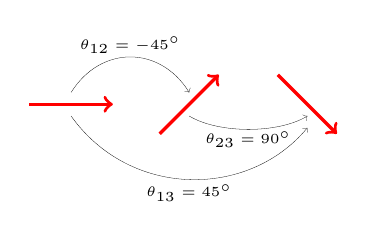
\begin{tikzpicture}[scale=1.5, font=\tiny]

\draw[->, very thick, red] (-0.3536, 0) -- (0.3536, 0);
\draw[->, very thick, red] (0.75, -0.25) -- (1.25, 0.25);
\draw[->, very thick, red] (1.75, 0.25) -- (2.25, -0.25);

\draw [ultra thin, ->](0,0.1) .. controls (0.25, 0.5) and (0.75, 0.5) .. (1,0.1);
\draw[ultra thin, ->] (1,-0.1) .. controls (1.25, -0.25) and (1.75, -0.25) .. (2,-0.1);
\draw[ultra thin, ->] (0,-0.1) .. controls (0.5, -0.8) and (1.5, -0.8) .. (2,-0.2);

\node at (0.5,0.5) { $\theta_{12} = -45^{\circ}$};
\node at (1.5,-0.3) { $\theta_{23} = 90^{\circ}$};
\node at (1,-0.75) { $\theta_{13} = 45^{\circ}$};


\end{tikzpicture}

\newpage

\noindent
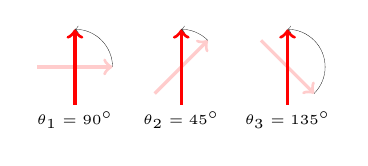
\begin{tikzpicture}[scale=1.35, font=\tiny]

\draw[->, very thick, red!20] (-0.3536, 0) -- (0.3536, 0);
\draw[->, very thick, red!20] (0.75, -0.25) -- (1.25, 0.25);
\draw[->, very thick, red!20] (1.75, 0.25) -- (2.25, -0.25);

\draw[->, very thick, red] (0, -0.3536) -- (0, 0.3536);
\draw[->, very thick, red] (1, -0.3536) -- (1, 0.3536);
\draw[->, very thick, red] (2, -0.3536) -- (2, 0.3536);

\draw [ultra thin, ->] (0.3536, 0)  arc (0:90:0.3536);
\draw [ultra thin, ->] (1.25, 0.25)  arc (45:90:0.3536);
\draw [ultra thin, ->] (2.25, -0.25)  arc (-45:90:0.3536);

\node at (0, -0.5) { $\theta_{1} = 90^{\circ}$};
\node at (1, -0.5) { $\theta_{2} = 45^{\circ}$};
\node at (2, -0.5) { $\theta_{3} = 135^{\circ}$};

\end{tikzpicture}

\end{document}